\documentclass[11pt]{article}
\usepackage[sc]{mathpazo} %Like Palatino with extensive math support
\usepackage{fullpage}
\usepackage[authoryear,sectionbib,sort]{natbib}
\linespread{1.7}
\usepackage[utf8]{inputenc}
\usepackage{lineno}
\usepackage{titlesec}
\titleformat{\section}[block]{\Large\bfseries\filcenter}{\thesection}{1em}{}
\titleformat{\subsection}[block]{\Large\itshape\filcenter}{\thesubsection}{1em}{}
\titleformat{\subsubsection}[block]{\large\itshape}{\thesubsubsection}{1em}{}
\titleformat{\paragraph}[runin]{\itshape}{\theparagraph}{1em}{}[. ]
\usepackage{fancyhdr}
\pagestyle{fancy}
\usepackage{geometry}
\usepackage{graphicx}
\usepackage[T1]{fontenc}
\usepackage[utf8]{inputenc}
\usepackage{authblk}
\usepackage{setspace}
\usepackage{amsfonts,amssymb,amsmath,hyperref}
\usepackage{float}
\usepackage{caption}
\usepackage{multirow}
\usepackage{hyperref}
\usepackage{wrapfig}
\usepackage{rotating}
\usepackage[usenames,dvipsnames]{xcolor}

%%%%%%%%%%%%%%%%%%%%%
% Header
%%%%%%%%%%%%%%%%%%%%%
%
% Customize the line below with the last name of your first author and
% the short title of your MS. You can comment authorship information out
% while your MS is undergoing double-blind review.
%
\rhead{Supplement to Miller and Compagnoni, ``Two-sex range limits'' \textit{Am.~Nat.}}
\setlength{\headsep}{0.3in}  
\lhead{} 

%%%%%%%%%%%%%%%%%%%%%
% Line numbering
%%%%%%%%%%%%%%%%%%%%%
%
% Please use line numbering with your initial submission and
% subsequent revisions. After acceptance, please turn line numbering
% off by adding percent signs to the lines %\usepackage{lineno} and
% to %\linenumbers{} and %\modulolinenumbers[3] below.
%
% To avoid line numbering being thrown off around math environments,
% the math environments have to be wrapped using
% \begin{linenomath*} and \end{linenomath*}
%
% (Thanks to Vlastimil Krivan for pointing this out to us!)

\title{Online Supplement: Two-sex demography, sexual niche differentiation, and the geographic range limits of Texas bluegrass (\textit{Poa arachnifera})\\ 
\LaTeX{} Template for Author-Supplied Supplementary PDFs, \\ 
\textit{The~American~Naturalist} }

% This version of the LaTeX supplementary template was last updated on
% November 8, 2019.

%%%%%%%%%%%%%%%%%%%%%
% Authorship
%%%%%%%%%%%%%%%%%%%%%
% Please remove authorship information while your paper is under review,
% unless you wish to waive your anonymity under double-blind review. You
% will need to add this information back in to your final files after
% acceptance.
%
% Once accepted for publication, author-supplied PDFs should have a 
% title page that includes (at least) the authors' names, the title of 
% the MS, and the name of the journal. It should also have a header and
% page numbers.

\author{Tom E.X. Miller$^{1,\ast}$ and Aldo Compagnoni$^{2,3}$} 
\date{}
\IfFileExists{upquote.sty}{\usepackage{upquote}}{}
\begin{document}
	\maketitle
	\noindent{} 1. Program in Ecology and Evolutionary Biology, Department of BioSciences, Rice University, Houston, TX 77005;
	\noindent{} 2. Institute of Biology, Martin Luther University Halle-Wittenberg, Halle, Germany;
	\noindent{} 3. German Centre for Integrative Biodiversity Research (iDiv), Leipzig, Germany;
	\noindent{} $\ast$ Corresponding author; e-mail: tom.miller@rice.edu



% In many cases, The American Naturalist allows authors to typeset their
% own supplementary material in an author-supplied PDF. This template
% applies to such cases. 
% 
% For appendices that will be typeset by the AmNat editorial staff, 
% please see the main LaTeX template, available from
% https://www.journals.uchicago.edu/journals/an/instruct
% Such appendices typically include descriptions of methods and tables
% defining parameters.
%
% In general, you have wide discretion for how you want to format an
% author-supplied PDF. They should in any case have a title page, 
% page numbers, and a header identifying the MS's (short) title.
%
% Counters for the online supplement should normally begin with an S
% (thus normally figure S1, figure S2, table S1, equation S1, etc.).

\renewcommand{\theequation}{S\arabic{equation}}
% redefine the command that creates the equation number.
\renewcommand{\thetable}{S\arabic{table}}
\renewcommand{\thesection}{S\arabic{section}}
\renewcommand{\thefigure}{S\arabic{figure}}
\setcounter{equation}{0}  % reset counter 
\setcounter{figure}{0}
\setcounter{table}{0}

% In online supplementary PDFs, sections can be numbered or not
% (at your discretion). If they are numbered, sections should usually
% begin with an S.

\newpage{}
\section*{Appendix A: Site locations and climate}
\renewcommand{\thefigure}{A\arabic{figure}}\setcounter{figure}{0}
\renewcommand{\thetable}{A\arabic{table}}\setcounter{table}{0}
\renewcommand{\theequation}{A\arabic{equation}}\setcounter{equation}{0}

% latex table generated in R 4.0.3 by xtable 1.8-4 package
% Mon Jan 17 20:32:35 2022
\begin{table}[ht]
	\centering
	\begin{tabular}{rlrrll}
		\hline
		& Population & Latitude & Longitude & Year\_visited & Experimental\_source \\ 
		\hline
		1 & Canyon\_of\_Eagles & 30.88 & -98.43 & 2012 & no \\ 
		2 & ClearBay-Thunderbird & 35.23 & -97.24 & 2013 & no \\ 
		3 & CooperWMA & 36.60 & -99.51 & 2012 & yes \\ 
		4 & Copper Breaks & 34.10 & -99.75 & 2013 & yes \\ 
		5 & Dinosaur\_Valley & 32.25 & -97.82 & 2012 & no \\ 
		6 & Fort\_Worth\_Nature\_Center & 32.83 & -97.46 & 2012 & no \\ 
		7 & Ft Cobb & 35.18 & -98.45 & 2013 & no \\ 
		8 & Ft Richardson & 33.20 & -98.16 & 2013 & no \\ 
		9 & Great Plains & 34.74 & -98.97 & 2013 & no \\ 
		10 & Great\_Salt\_Plains & 36.79 & -98.18 & 2012 & no \\ 
		11 & Horn\_Hill\_Cemetery & 31.56 & -96.64 & 2012 & yes \\ 
		12 & Kingman\_Fishing\_Lake & 37.65 & -98.28 & 2012 & no \\ 
		13 & Lake Arrowhead & 33.75 & -98.39 & 2013 & yes \\ 
		14 & Mineral\_Wells & 32.89 & -98.01 & 2012 & no \\ 
		15 & Pedernales\_Falls & 30.33 & -98.25 & 2012 & no \\ 
		16 & Possum Kingdom & 32.87 & -98.57 & 2013 & no \\ 
		17 & Quartz\_Mountain & 34.89 & -99.30 & 2012 & yes \\ 
		18 & Red Rock Canyon & 35.44 & -98.35 & 2013 & no \\ 
		19 & Red\_River & 34.13 & -98.10 & 2012 & no \\ 
		20 & South\_Llano & 30.45 & -99.80 & 2012 & yes \\ 
		21 & Sulfur\_Springs & 31.08 & -98.46 & 2012 & yes \\ 
		22 & Wichita\_Mountains & 34.70 & -98.67 & 2012 & no \\ 
		\hline
	\end{tabular}
	\caption{Sites of natural population surveys} 
	\label{tab:survey}
\end{table}


\clearpage
% latex table generated in R 4.0.3 by xtable 1.8-4 package
% Mon Jan 17 20:32:35 2022
\begin{sidewaystable}[ht]
	\centering
	\begin{tabular}{rllrr}
		\hline
		& Site & City, State & Latitude & Longitude \\ 
		\hline
		1 & Buffalo Lake National Wildlife Refuge & Amarillo, TX & 35.20 & -101.85 \\ 
		2 & USDA-ARS Grazinglands Research Laboratory & El Reno, OK & 35.53 & -97.96 \\ 
		3 & Katy Prairie Conservatory Indiangrass Preserve & Waller, TX & 29.92 & -95.92 \\ 
		4 & Texas Tech University Llano River Research Station & Junction, TX & 30.49 & -99.77 \\ 
		5 & Lake Lewisville Environmental Learning Area & Lewisville, TX & 33.07 & -96.96 \\ 
		6 & University of Texas Stengl Lost Pines Biological Station & Bastrop, TX & 30.18 & -97.47 \\ 
		7 & Texas Tech University & Lubbock, TX & 33.57 & -101.88 \\ 
		8 & Wichita State University Ninnescah Field Station & Wichita, KS & 37.54 & -97.67 \\ 
		9 & Texas A\&M AgriLife Research and Extension Center & Ozona, TX & 30.71 & -101.20 \\ 
		10 & Pittsburgh State University Field Station & Pittsburgh, KS & 37.41 & -94.70 \\ 
		11 & Sam Houston State University Center for Biological Field Studies & Huntsville, TX & 30.72 & -95.55 \\ 
		12 & Texas A\&M AgriLife Research and Extension Center & Vernon, TX & 34.15 & -99.29 \\ 
		13 & River Bend Nature Center & Wichita Falls, TX & 33.91 & -98.51 \\ 
		14 & USDA-ARS Range and Pature Research & Woodward, OK & 36.43 & -99.40 \\ 
		\hline
	\end{tabular}
	\caption{Sites of common garden experiments} 
	\label{tab:experiment}
\end{sidewaystable}


\newpage
\begin{figure}[h!]
	\begin{center}
		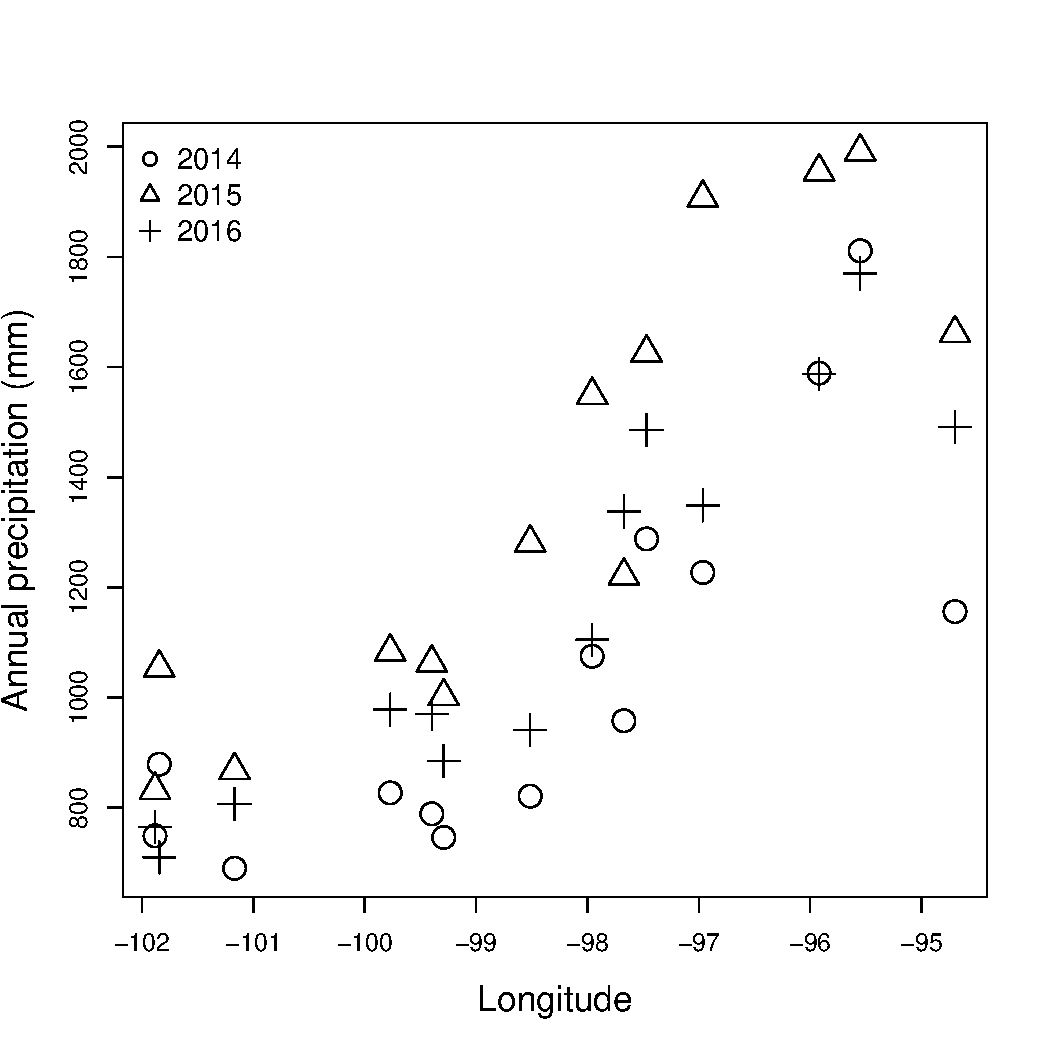
\includegraphics[width=0.75\linewidth]{Figures/site_precip}
		\caption{Total annual precipitation at common garden sites during the study years tracked long-term trends of increasing aridity from east to west.}
		\label{fig:site_precip}
	\end{center}
\end{figure}

%--------------------------------------------------------------------
\newpage
\section*{Appendix B: Additional results}
\renewcommand{\thefigure}{B\arabic{figure}}\setcounter{figure}{0}
\renewcommand{\thetable}{B\arabic{table}}\setcounter{table}{0}
\renewcommand{\theequation}{B\arabic{equation}}\setcounter{equation}{0}

\begin{figure}[H]
	\begin{center}
		\includegraphics[width=0.75\linewidth]{Figures/PPC}
		\caption{Posterior predictive checks of statistical models for demographic vital rates. 
			Lines show density distributions of real data (thick, dark blue) compared to simulated data sets (thin, light blue) generated from the fitted models based on 500 draws of the posterior distribution of parameter estimates. 
			Correspondence of the real and simulated data suggests that the fitted models describe the data well.}
		\label{fig:PPC}
	\end{center}
\end{figure}

\newpage
\begin{figure}[H]
	\begin{center}
		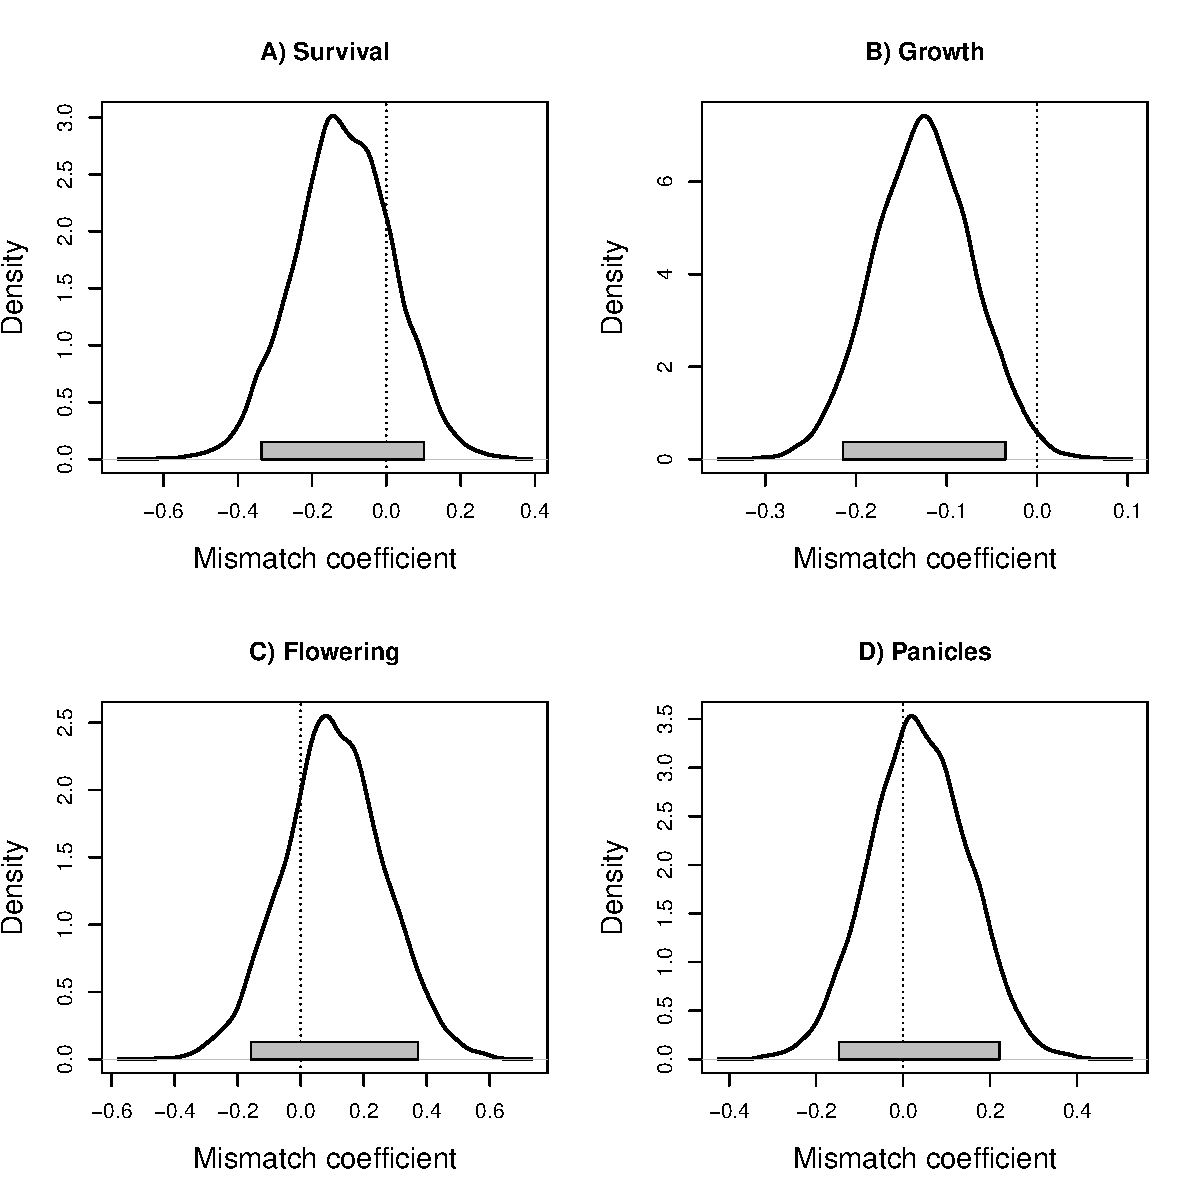
\includegraphics[width=0.75\linewidth]{Figures/climate_mismatch}
		\caption{Posterior distributions of statistical coefficients for the influence of source-garden climate mismatch on survival (A), growth (B), flowering (C), and panicle production (D). Gray bars show the 95\% credible interval of the coefficients. Climate mismatch was calculated as the absolute value of the difference in mean annual precipitation between source population and common garden location.}
		\label{fig:climate_mismatch}
	\end{center}
\end{figure}

\newpage
\begin{figure}[H]
	\begin{center}
		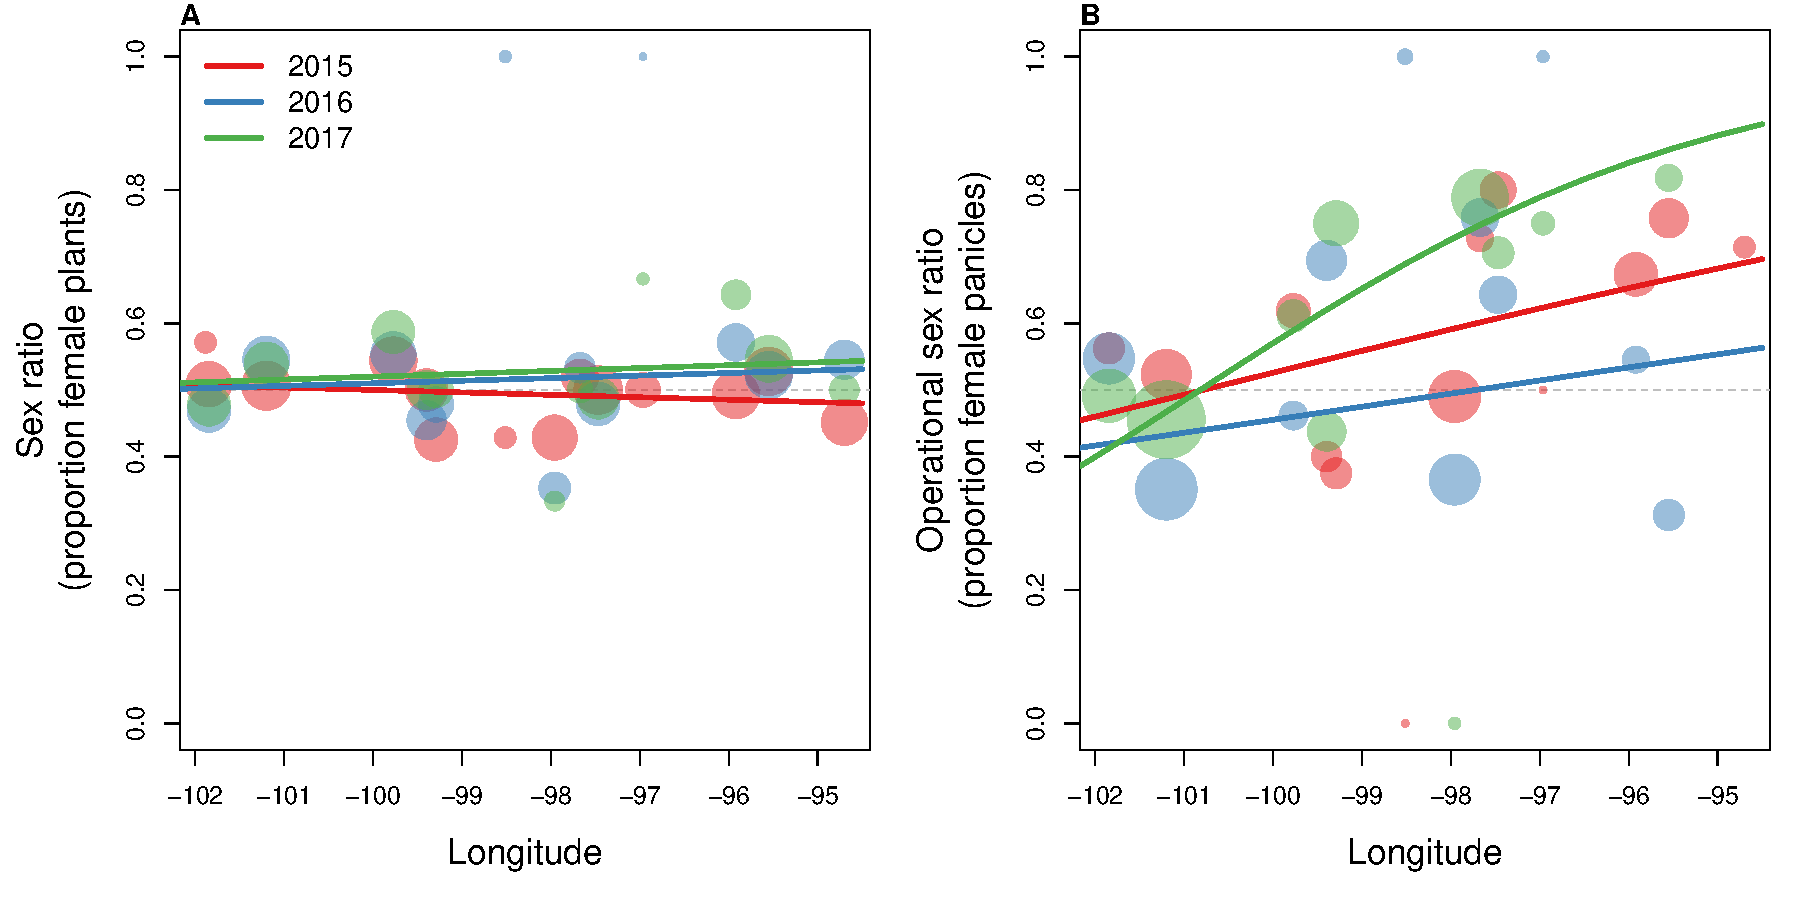
\includegraphics[width=0.75\linewidth]{Figures/garden_sex_ratios}
		\caption{Year-specific sex ratios of plants (A) and panicles (B) in common garden populations spanning the longitudinal aridity gradient. Points sizes are proportional to sample sizes and lines show fitted binomial GLMs.}
		\label{fig:gardens_by_year}
	\end{center}
\end{figure}

\newpage
\begin{figure}[H]
	\begin{center}
		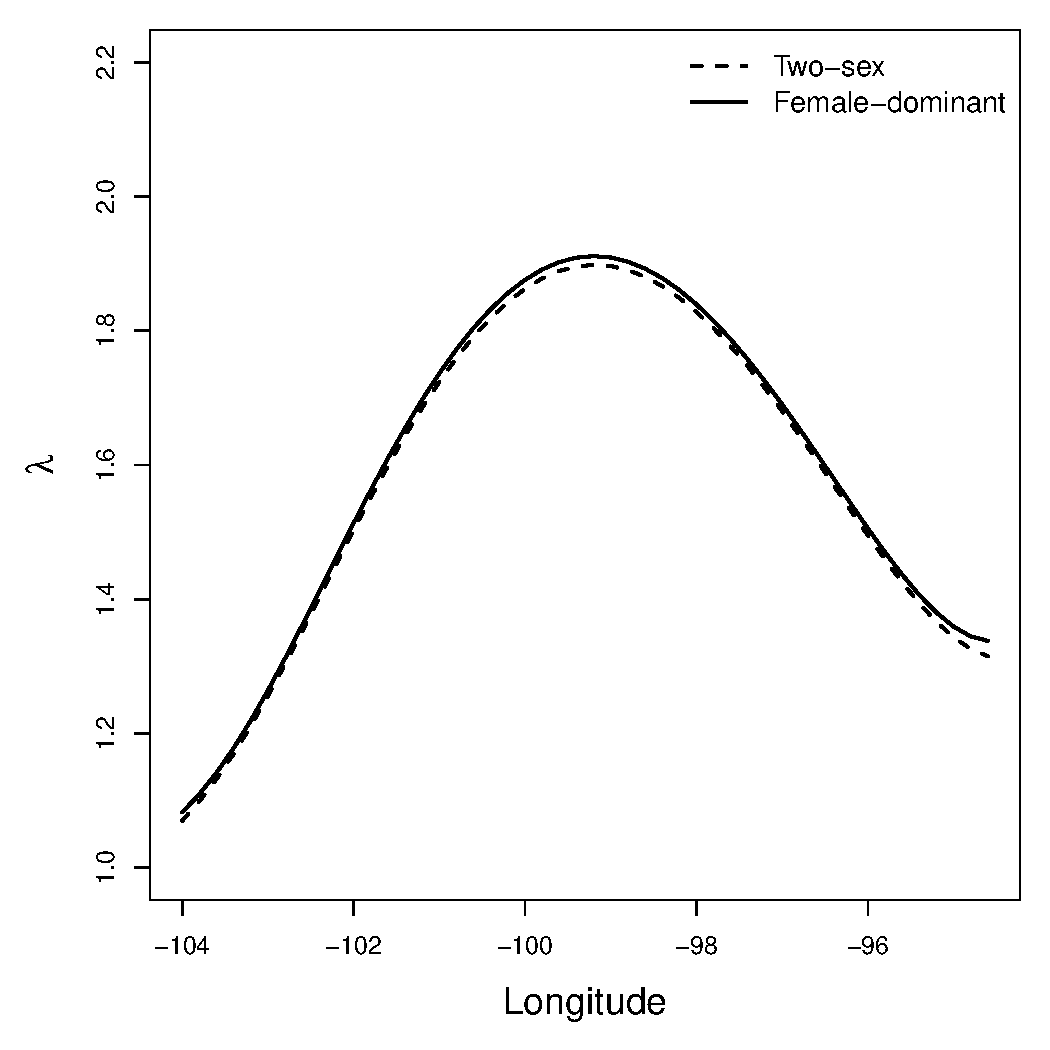
\includegraphics[width=0.75\linewidth]{Figures/lambda_long_2sex_Fdom}
		\caption{Comparison of longitudinal variation in $\lambda$ between the two-sex demographic model (dashed line) that includes dependence of female seed production on population structure and the corresponding female-dominant model (solid line) with constant female fertility and all else equal. 
			Models were evaluated at posterior mean parameter estimates}
		\label{fig:2sex_Fdom}
	\end{center}
\end{figure}

\newpage
\begin{figure}[H]
	\begin{center}
		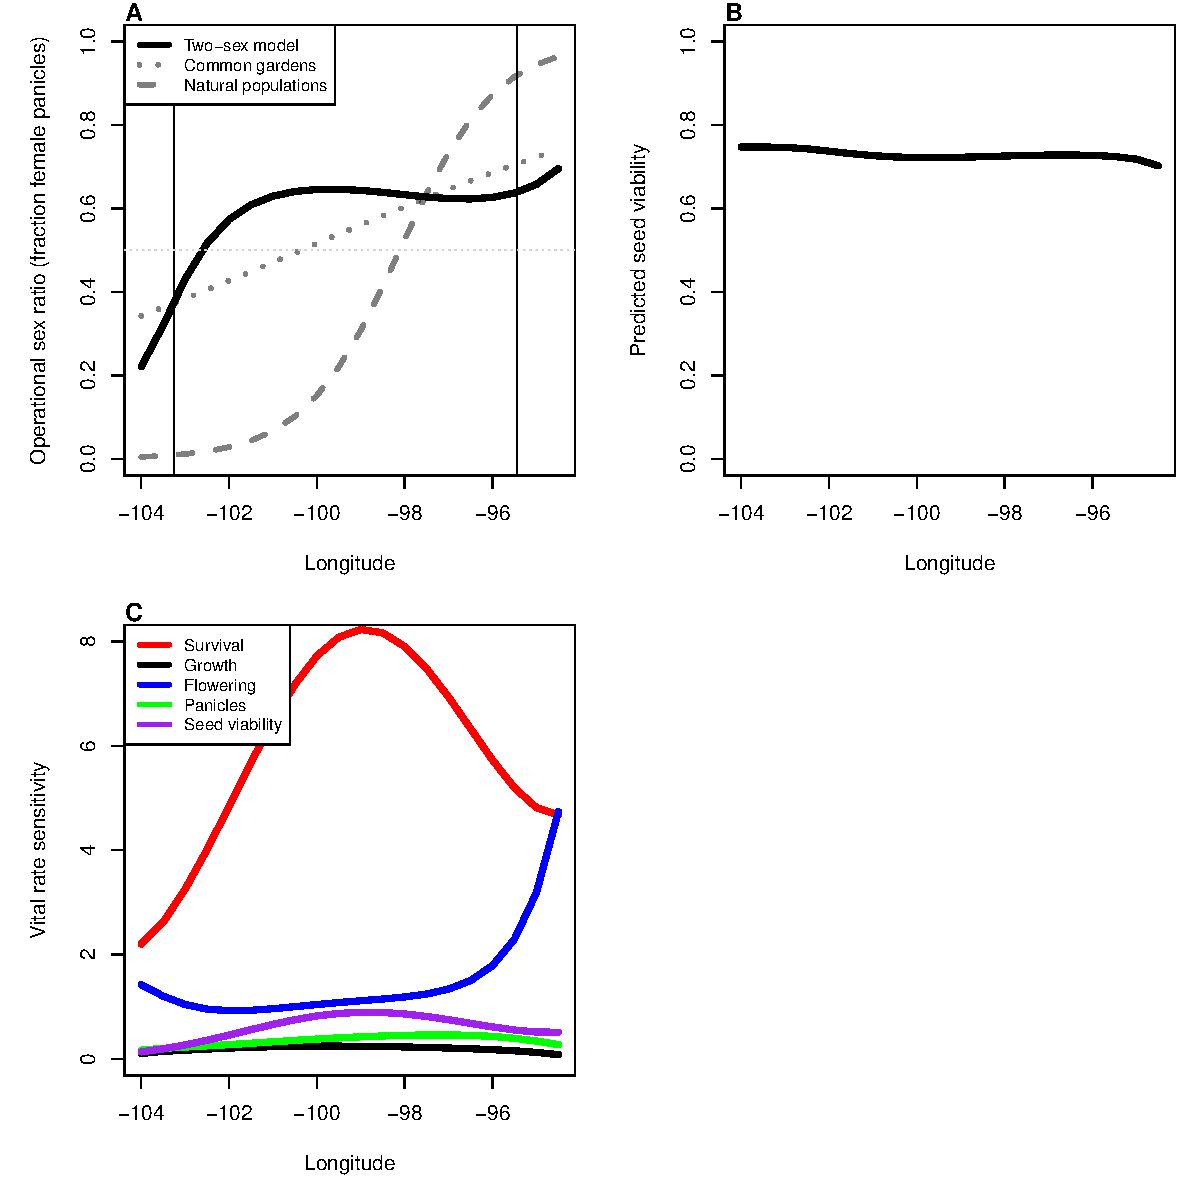
\includegraphics[width=\linewidth]{Figures/SR_viab_sens}
		\caption{\textbf{A}, Longitudinal variation in operational sex ratio (fraction of panicles that are female) predicted by the two-sex MPM (solid line) compared to the sex ratio clines fitted to data from common gardens (dotted line) or natural populations (dashed line).
			Vertical lines show the longitudes of the westernmost and easternmost counties with occurrence records of \textit{P. arachnifera}.
			\textbf{B}, Longitudinal variation in seed viability predicted by the two-sex MPM according to Eq. 4 and the OSR variation shown in \textbf{A}.
			\textbf{C}, Sensitivities of $\lambda$ to vital rates in relation to longitude.
			Sensitivities were calculated numerically by perturbing vital rate functions (across all sizes) by $0.01$, recalculating $\lambda$, and dividing the difference by $0.01$.
			Vital rates were perturbed equally for both sexes though results in Fig \ref{fig:lambda_long}B,C suggest that vital rate sensitivities were dominated by females. 
		}
		\label{fig:SR_viab_sens}
	\end{center}
\end{figure}

\newpage
% latex table generated in R 4.0.3 by xtable 1.8-4 package
% Mon Jan 17 20:32:35 2022
\begin{table}[ht]
	\centering
	\begin{tabular}{rlrrr}
		\hline
		& Model & WAIC & ELPD & SE(ELPD) \\ 
		\hline
		1 & Climate & 13286.29 & -6643.14 & 87.46 \\ 
		2 & Longitude & 13288.39 & -6644.19 & 87.25 \\ 
		\hline
	\end{tabular}
	\caption{Model selection results for candidate vital rate models with longitude or climate (mean annual precipitation) as environmental covariates. Table shows WAIC (Watanabe-Akaike Information Criterion), ELPD (expected log predictive density), and the standard error of ELPD. The fact that the SE of ELPD is much greater than the difference between models suggests that longitude and climate are effectively interchangeable as environmental covariates.} 
	\label{tab:waic}
\end{table}

%--------------------------------------------------------------------
\newpage
\section*{Appendix C: Size distribution comparisons and simulation experiments}
\renewcommand{\thefigure}{C\arabic{figure}}\setcounter{figure}{0}
\renewcommand{\thetable}{C\arabic{table}}\setcounter{table}{0}
\renewcommand{\theequation}{C\arabic{equation}}\setcounter{equation}{0}

In this section, we compare size distributions of natural and experimental populations, and explore how the size distribution predicted by the two-sex MPM affects our conclusions about the role of males in range boundary formation. 

\subsection*{Observed and predicted size distributions}

\paragraph{Natural populations}
During natural population surveys (2012--2013) we recorded the area ($m^2$) of Texas bluegrass patches using a Trimble GeoExplorer hand-held GPS receiever with sub-meter accuracy. 

\paragraph{Common garden populations}
Common garden data collection included tiller counts and the maximum length and width of each patch, which we converted to area ($m^2$) assuming an oval shape. 
We used these data to estimate the relationship between patch area and tiller count (Fig. \ref{fig:area_tillers_conversion}) using a generalized additive model \citep{mgcv} and applied this fitted relationship to area measurements from natural populations.
This allowed us to compare the size distributions of natural and common garden populations (pooled across the range) in the same size unit (log(tillers)).

\newpage
\begin{figure}[H]
	\begin{center}
		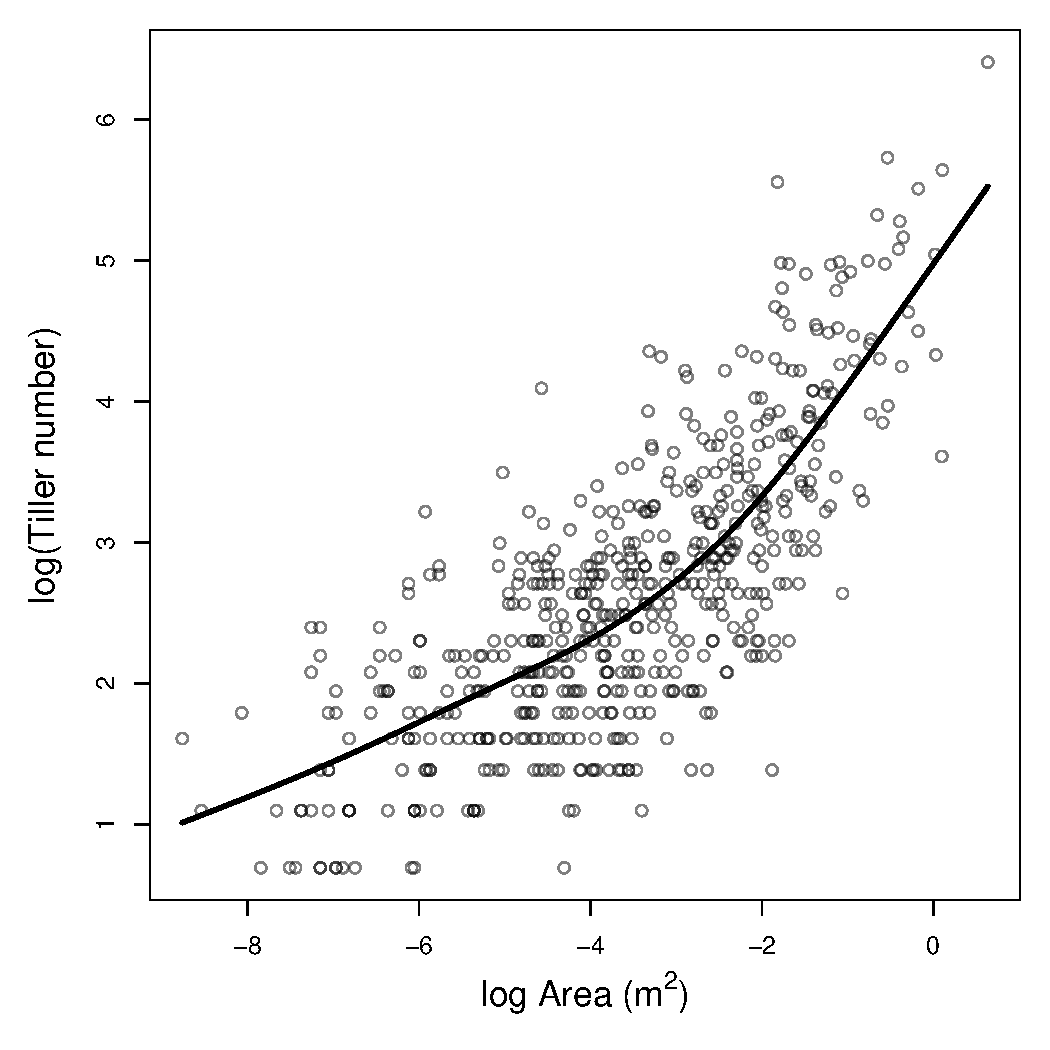
\includegraphics[width=0.75\linewidth]{Figures/area_tillers_conversion}
		\caption{Relationship between area ($m^2$) and tiller count from plants in the common garden experiment. 
			The fitted gam model (line) was used to convert area measurements from natural populations to tiller counts.}
		\label{fig:area_tillers_conversion}
	\end{center}
\end{figure}

\paragraph{Two-sex MPM}
The two-sex MPM predicts asymptotic population structure, including stable size distribution (SSD) and sex ratio. 
For comparison with empirical data, we calculated the SSD (pooling both sexes) predicted in the center of the range (the conclusions that we draw from this analysis hold up if we consider SSD from different parts of the range).
Because the MPM is structured by tiller number, we converted the SSD to log(tillers) by simulating an arbirarily large ($10000$) population at SSD, taking the natural logarithm of tiller number, and then estimating the empirical distribution of this variable. 

\newpage
\begin{figure}[H]
	\begin{center}
		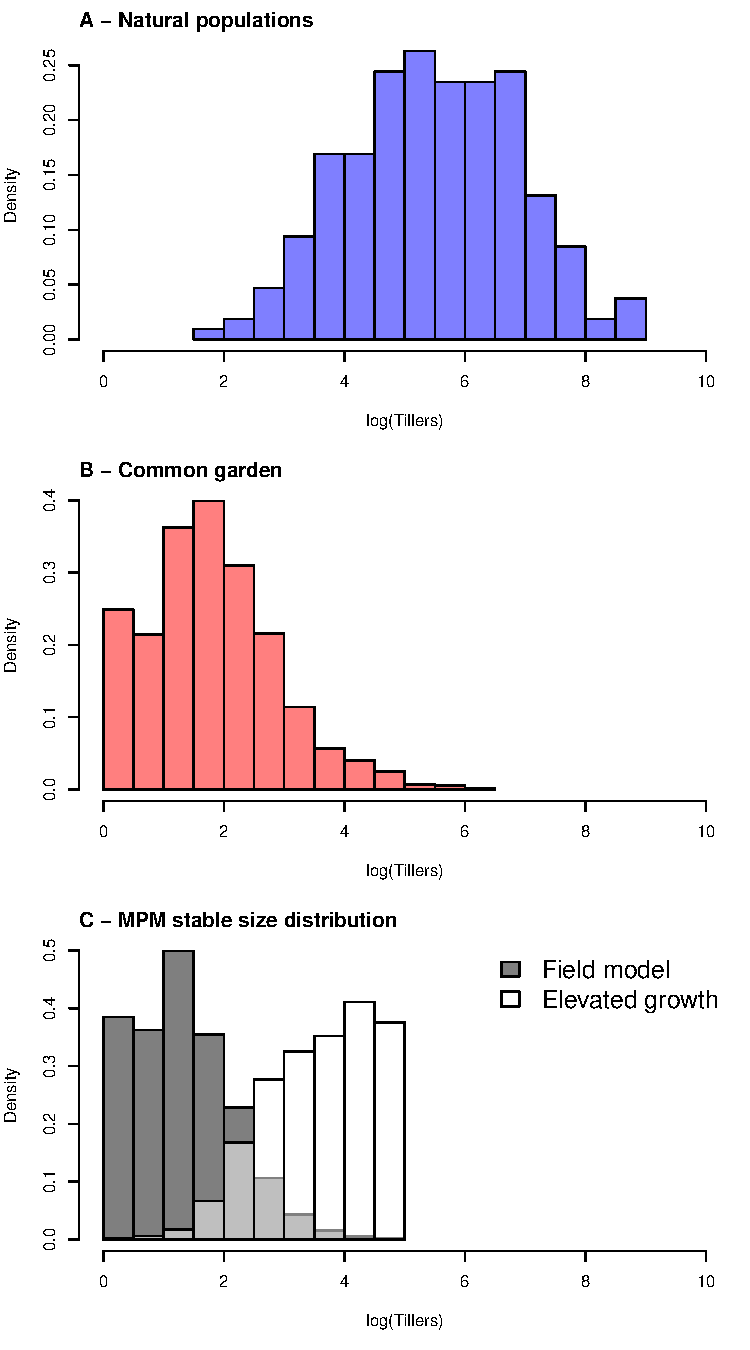
\includegraphics[width=0.5\linewidth]{Figures/size_dist}
		\caption{Size distribution of Texas bluegrass from natural populations (\textbf{A}), common garden populations (\textbf{B}), and predicted by the two-sex MPM (\textbf{C}). 
			In \textbf{C}, the two size distributions come from the base model parameterized following methods described in the main manuscript (``field model'', in gray) and a numerical experiment where growth parameters were numerically increased to generate a size distribution more consistent with natural populations (``elevated growth model'', in white). 
		}
		\label{fig:size_dist}
	\end{center}
\end{figure}

\paragraph{Results}
Plants from natural populations were larger, on average, than plants in our common garden experiment (Fig. \ref{fig:size_dist}A,B).
Common garden plants were generally larger each year but the largest sizes in the final year of the common garden corresponded to smaller sizes observed in natural populations (although natural population surveys were subject to detection bias: small plants were likely under-sampled relative to their occurrence). 
The predicted SSD from the two-sex MPM was consistent with the common garden size distribution (Fig. \ref{fig:size_dist}C), as expected since the model was built with common garden data. 
These results suggest that common garden plants did not have the same growth trajectories of naturally occurring plants and / or were not given sufficient time to reach the sizes observed in natural populations. 

\subsection*{Numerical experiment to explore the consequences of under-estimating the size distribution}
The preceding results indicate that the common garden populations, and thus the two-sex MPM built from common garden data, under-estimate the size distribution of Texas bluegrass, relative to what we find in natural populations. 
Sex differences in demography, and especially flowering, were most pronounced for the largest sizes (Fig. 4), but these sizes were predicted to be very rare in a stable population (Fig. \ref{fig:size_dist}C). 
The under-estimation of large sizes may explain why longitudinal clines in OSR predicted by the MPM and seen in the common garden were weaker than the OSR cline observed in natural populations (Fig. \ref{fig:SR_viab_sens}). 
It is therefore possible that our main finding -- that males contribute little-to-nothing toward range limitation -- reflects a limitation of the model, since real populations tended to be more female-biased (and potentially more mate-limited) in the eastern range margins than the model predicted.
To explore this possibility, we conducted a numerical experiment that allowed modeled plants to reach larger sizes by increasing the empirically-estimated intercept of the growth vital rate function by a factor of $2.75$ (values larger than this caused numerical instabilities).
This adjustment caused all plants to increase in size more strongly regardless of initial size, sex, or geographic location. 
We also increased the upper size limit to $U*1.5$.

As expected, this led to stronger sex ratio clines and stronger reductions in seed viability at eastern range margins (Fig. \ref{fig:elevated_growth_SR_viab}). 
These changes increased the contributions of males to eastern range limitation in the elevated-growth numerical experiment.
However, the contribution of males to range limitation was still weak relative to that of females (the maximum male contribution was less than half of the female maximum) and differences between the two-sex and female-dominant MPMs were stil very minor (Fig. \ref{fig:elevated_growth_model}). 
Collectively, these results suggest that the small size distribution of the common garden experiment led to a weaker role of males than would be expected in populations with a more realistic size distribution, but that even with a larger size distribution, declines in female performance still dominante range boundary formation.

\begin{figure}[H]
	\begin{center}
		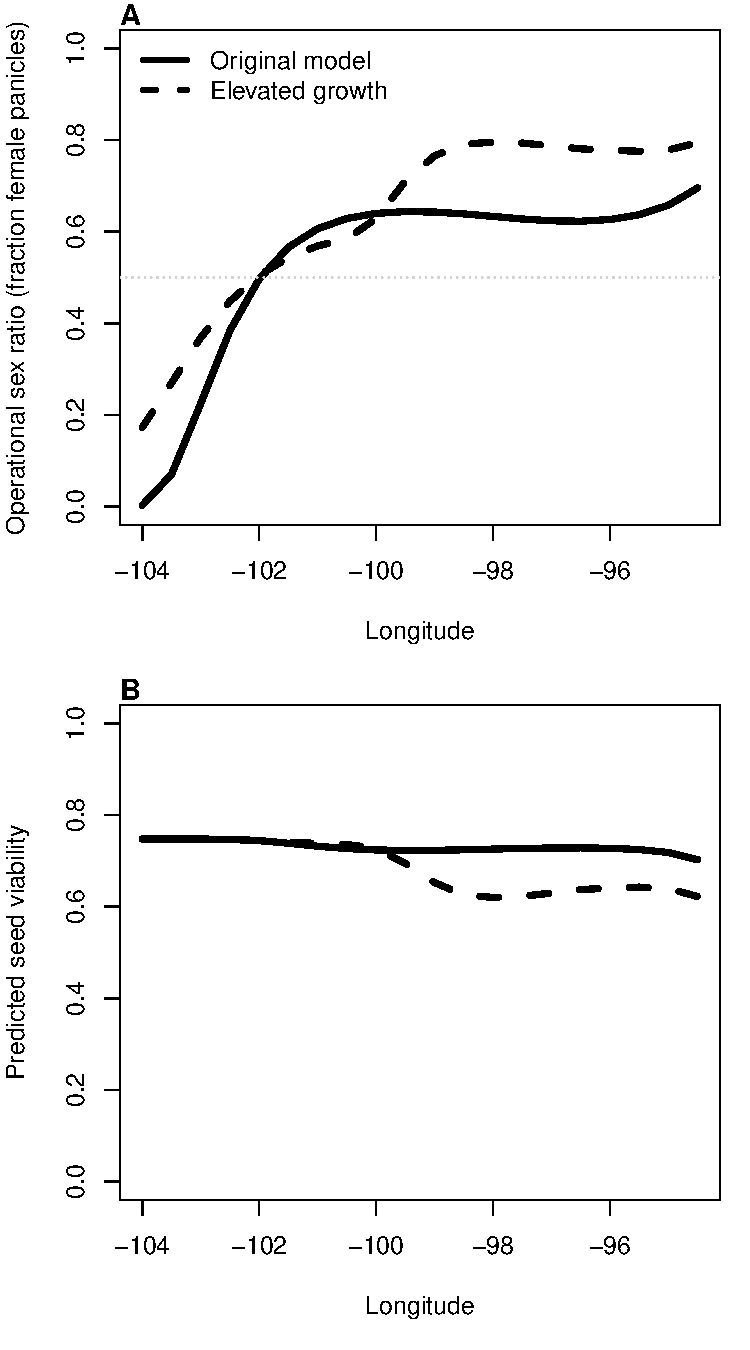
\includegraphics[width=0.5\linewidth]{Figures/elevated_growth_SR_viab}
		\caption{Two-sex model predictions for \textbf{A} operational sex ratio (fraction of panicles that are female) and \textbf{B} seed viability at stable population structure in relation to longitude. 
			Solid line shows predictions of the base model using field-estmated parameter values and dashed line shows the same model with elevated growth of both sexes and across all longitudes (intercept of growth function increased by a factor of 2.75). }
		\label{fig:elevated_growth_SR_viab}
	\end{center}
\end{figure}

\begin{figure}[H]
	\begin{center}
		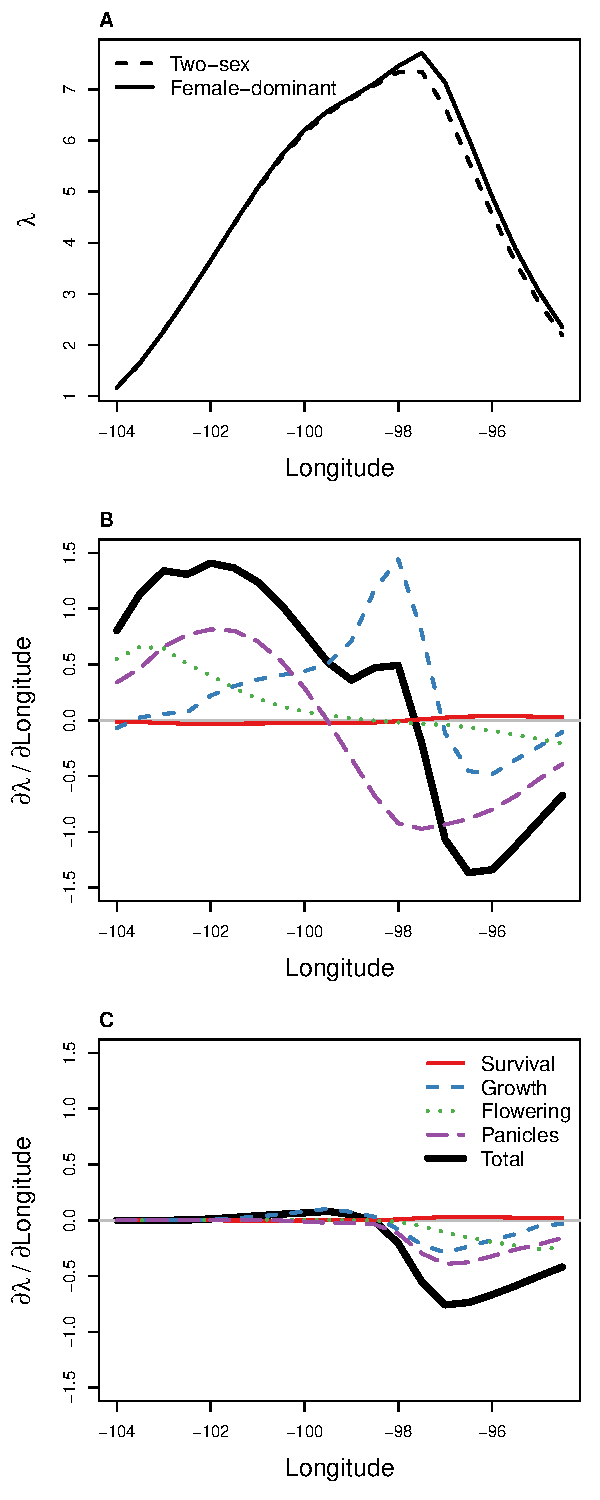
\includegraphics[width=0.5\linewidth]{Figures/elevated_growth_model}
		\caption{Results for the elevated growth model, in which the intercept of growth function was increased by a factor of 2.75.
			\textbf{A}, contrast of two-sex and female-dominant models, as in Fig. \ref{fig:2sex_Fdom};
			\textbf{B,C}, Life Table Response Experiments decomposing the change in $\lambda$ with respect to longitude into contributions from female \textbf{B} and male \textbf{C} vital rates (layout as in Fig. 6). 
		}
		\label{fig:elevated_growth_model}
	\end{center}
\end{figure}

%--------------------------------------------------------------------
\newpage
\bibliographystyle{apalike}
\bibliography{POAR_range_limits}

\end{document}
